\documentclass{beamer}
\usepackage{amsmath}
\usepackage{gvv}

\title{Question 4.4.36}
\author{AI25BTECH11040 - Vivaan Parashar}
\date{\today}

\begin{document}

\frame{\titlepage}

\begin{frame}
    \frametitle{Question: }
    The area of the triangle formed by the lines $\frac{x}{a} + \frac{y}{b} = 1$ and the coordinate axes is \underline{\hspace{2cm}}.
\end{frame}

\begin{frame}
    \frametitle{Solution: }
    Let the origin be $\vec{O}$, the x-intercept be $\vec{A}$, and the y-intercept be $\vec{B}$. We then need the area of triangle $OAB$.
The x-intercept is some multiple of the basis vector $\vec{e_1}$, and the y-intercept is some multiple of the basis vector $\vec{e_2}$. Thus,
\begin{align}
    \therefore \vec{O} = \myvec{0 \\ 0}, \quad \vec{A} = \lambda\vec{e_1}, \quad \vec{B} = \mu\vec{e_2}
\end{align}
The equation of the line can be written as
\begin{align}
    \vec{n}^{\mathrm{T}}\vec{x} = 1
\end{align}
Where $\vec{n} = \myvec{\frac{1}{a} \\ \frac{1}{b}}$, and $\vec{x}$ is any point on the line.
By putting the points $\vec{A}$ and $\vec{B}$ in the equation of the line, we get
\begin{align}
    \lambda\vec{n}^{\mathrm{T}}\vec{e_1} = 1, \quad \mu\vec{n}^{\mathrm{T}}\vec{e_2} = 1\\
    \implies \lambda = \frac{1}{\vec{n}^{\mathrm{T}}\vec{e_1}} = a, \quad \mu = \frac{1}{\vec{n}^{\mathrm{T}}\vec{e_2}} = b
\end{align}
\end{frame}
\begin{frame}
    Now,
\begin{align}
    \Delta\text{OAB} = \frac{1}{2}\left|\vec{A}\times\vec{B}\right|\\
    \implies \Delta\text{OAB} = \frac{1}{2} \lambda \mu \left|\vec{e_1}\times\vec{e_2}\right|\\
    \therefore \Delta\text{OAB} = \left|\frac{ab}{2}\right|
\end{align}
\end{frame}

\begin{frame}
    \frametitle{Plot: }
    \begin{figure}[h!]
        \centering
        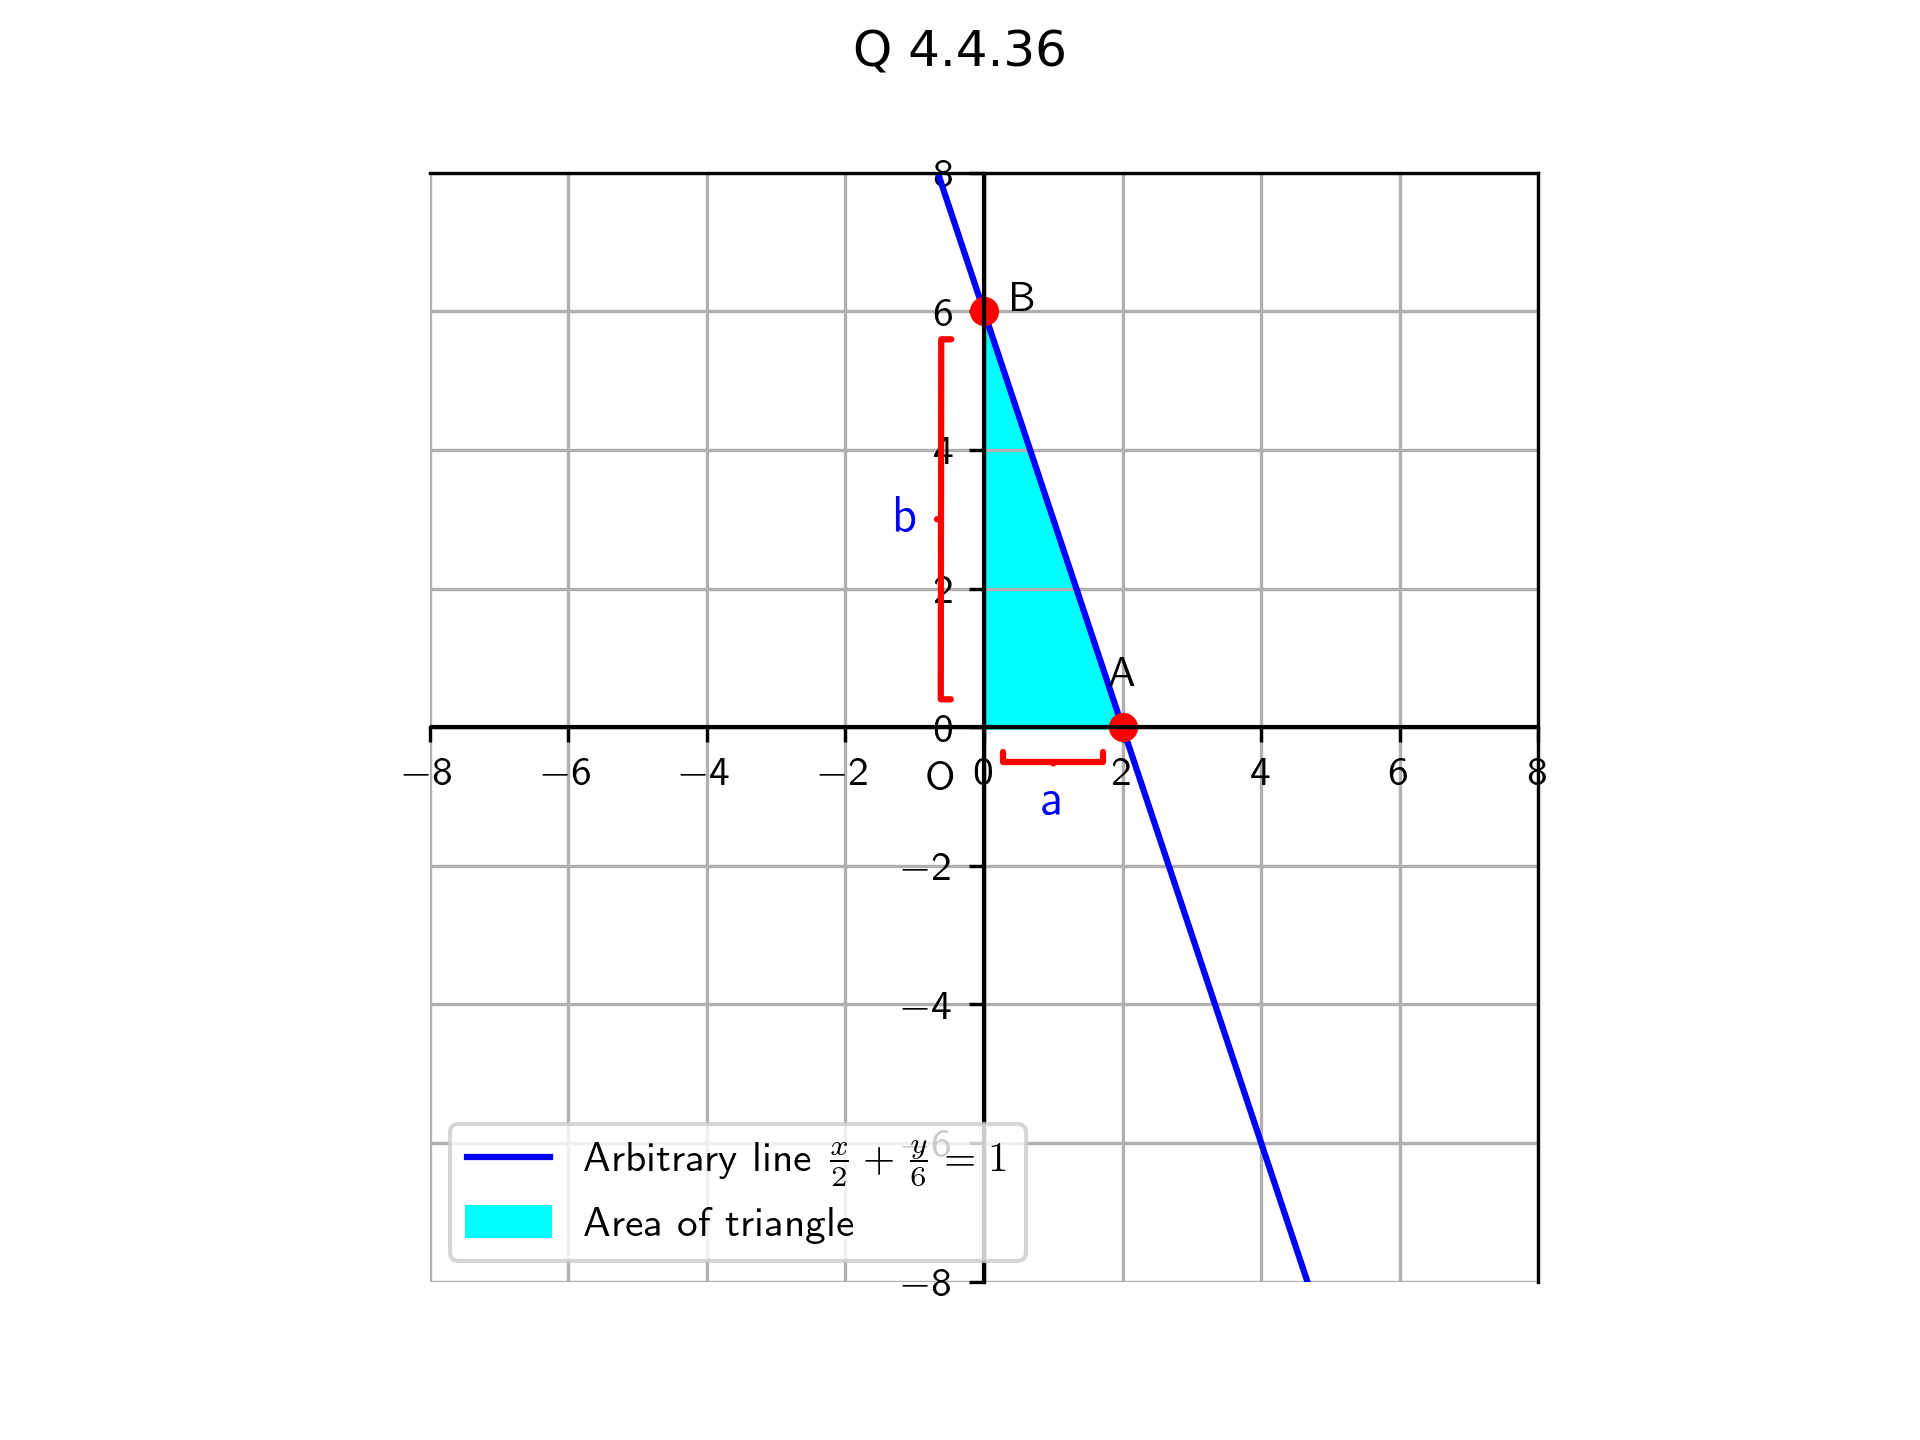
\includegraphics[width=0.9\columnwidth]{../figs/plot.png}
        \caption{Graph of line and triangle formed by intercepts with axes}
        \label{fig:4.4.36}
    \end{figure}
\end{frame}

\end{document}
